\newpage
\section{Конструкторская часть}

Рассмотрим алгоритм конвеерных вычислений для алгоритма Винограда.

\subsection{Функциональная модель}

На рисунке \ref{img:idef0} представлена функциональная модель IDEF0 уровня 1.

\begin{figure}[H]
    \center{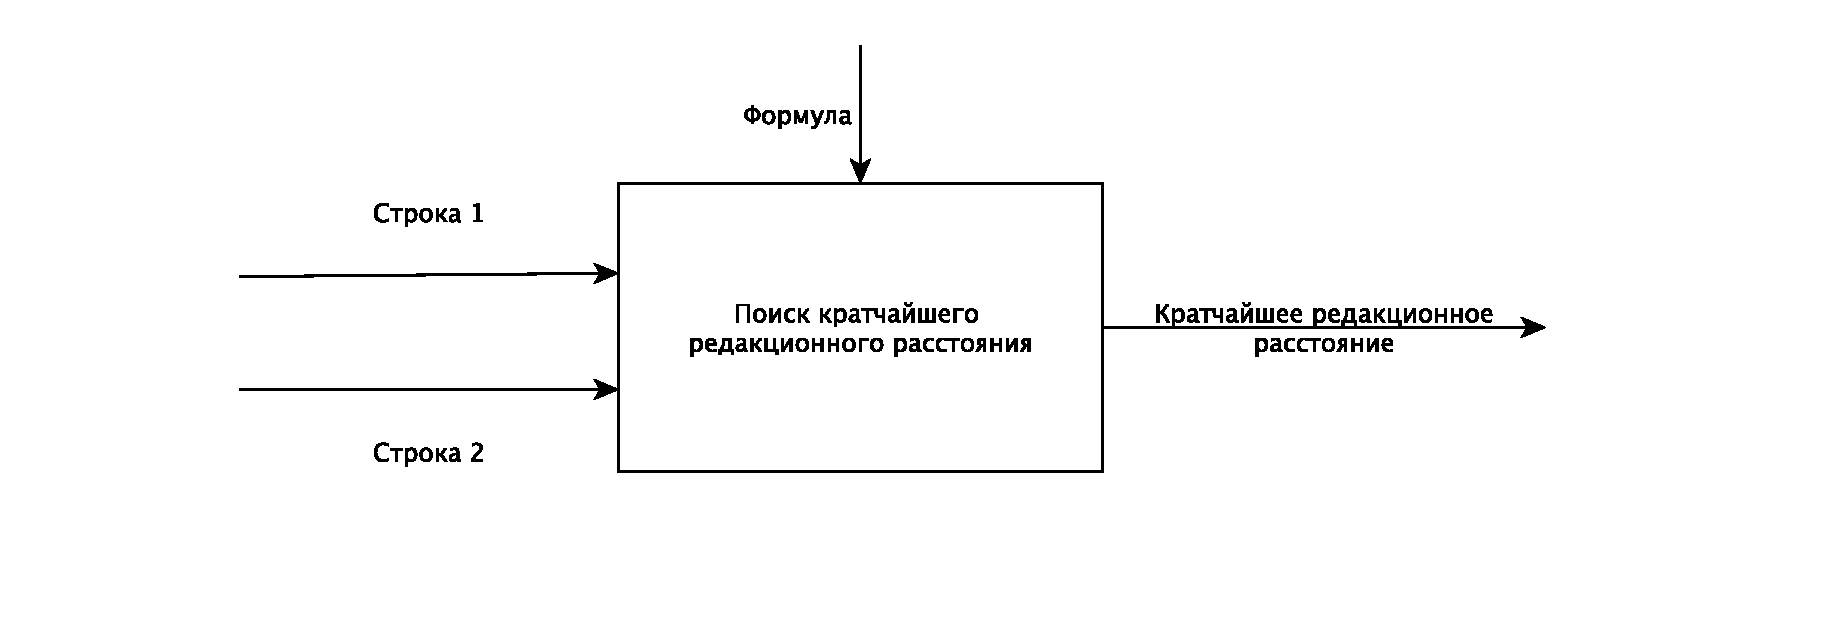
\includegraphics[scale=0.8]{IDEF0}}
    \caption{Функциональная модель IDEF0 уровня 1}
    \label{img:idef0}
\end{figure}

\subsection{Схемы алгоритмов}

На рисунке \ref{img:modvinograd} изображена схема
алгоритма Винограда.

\begin{figure}[H]
    \center{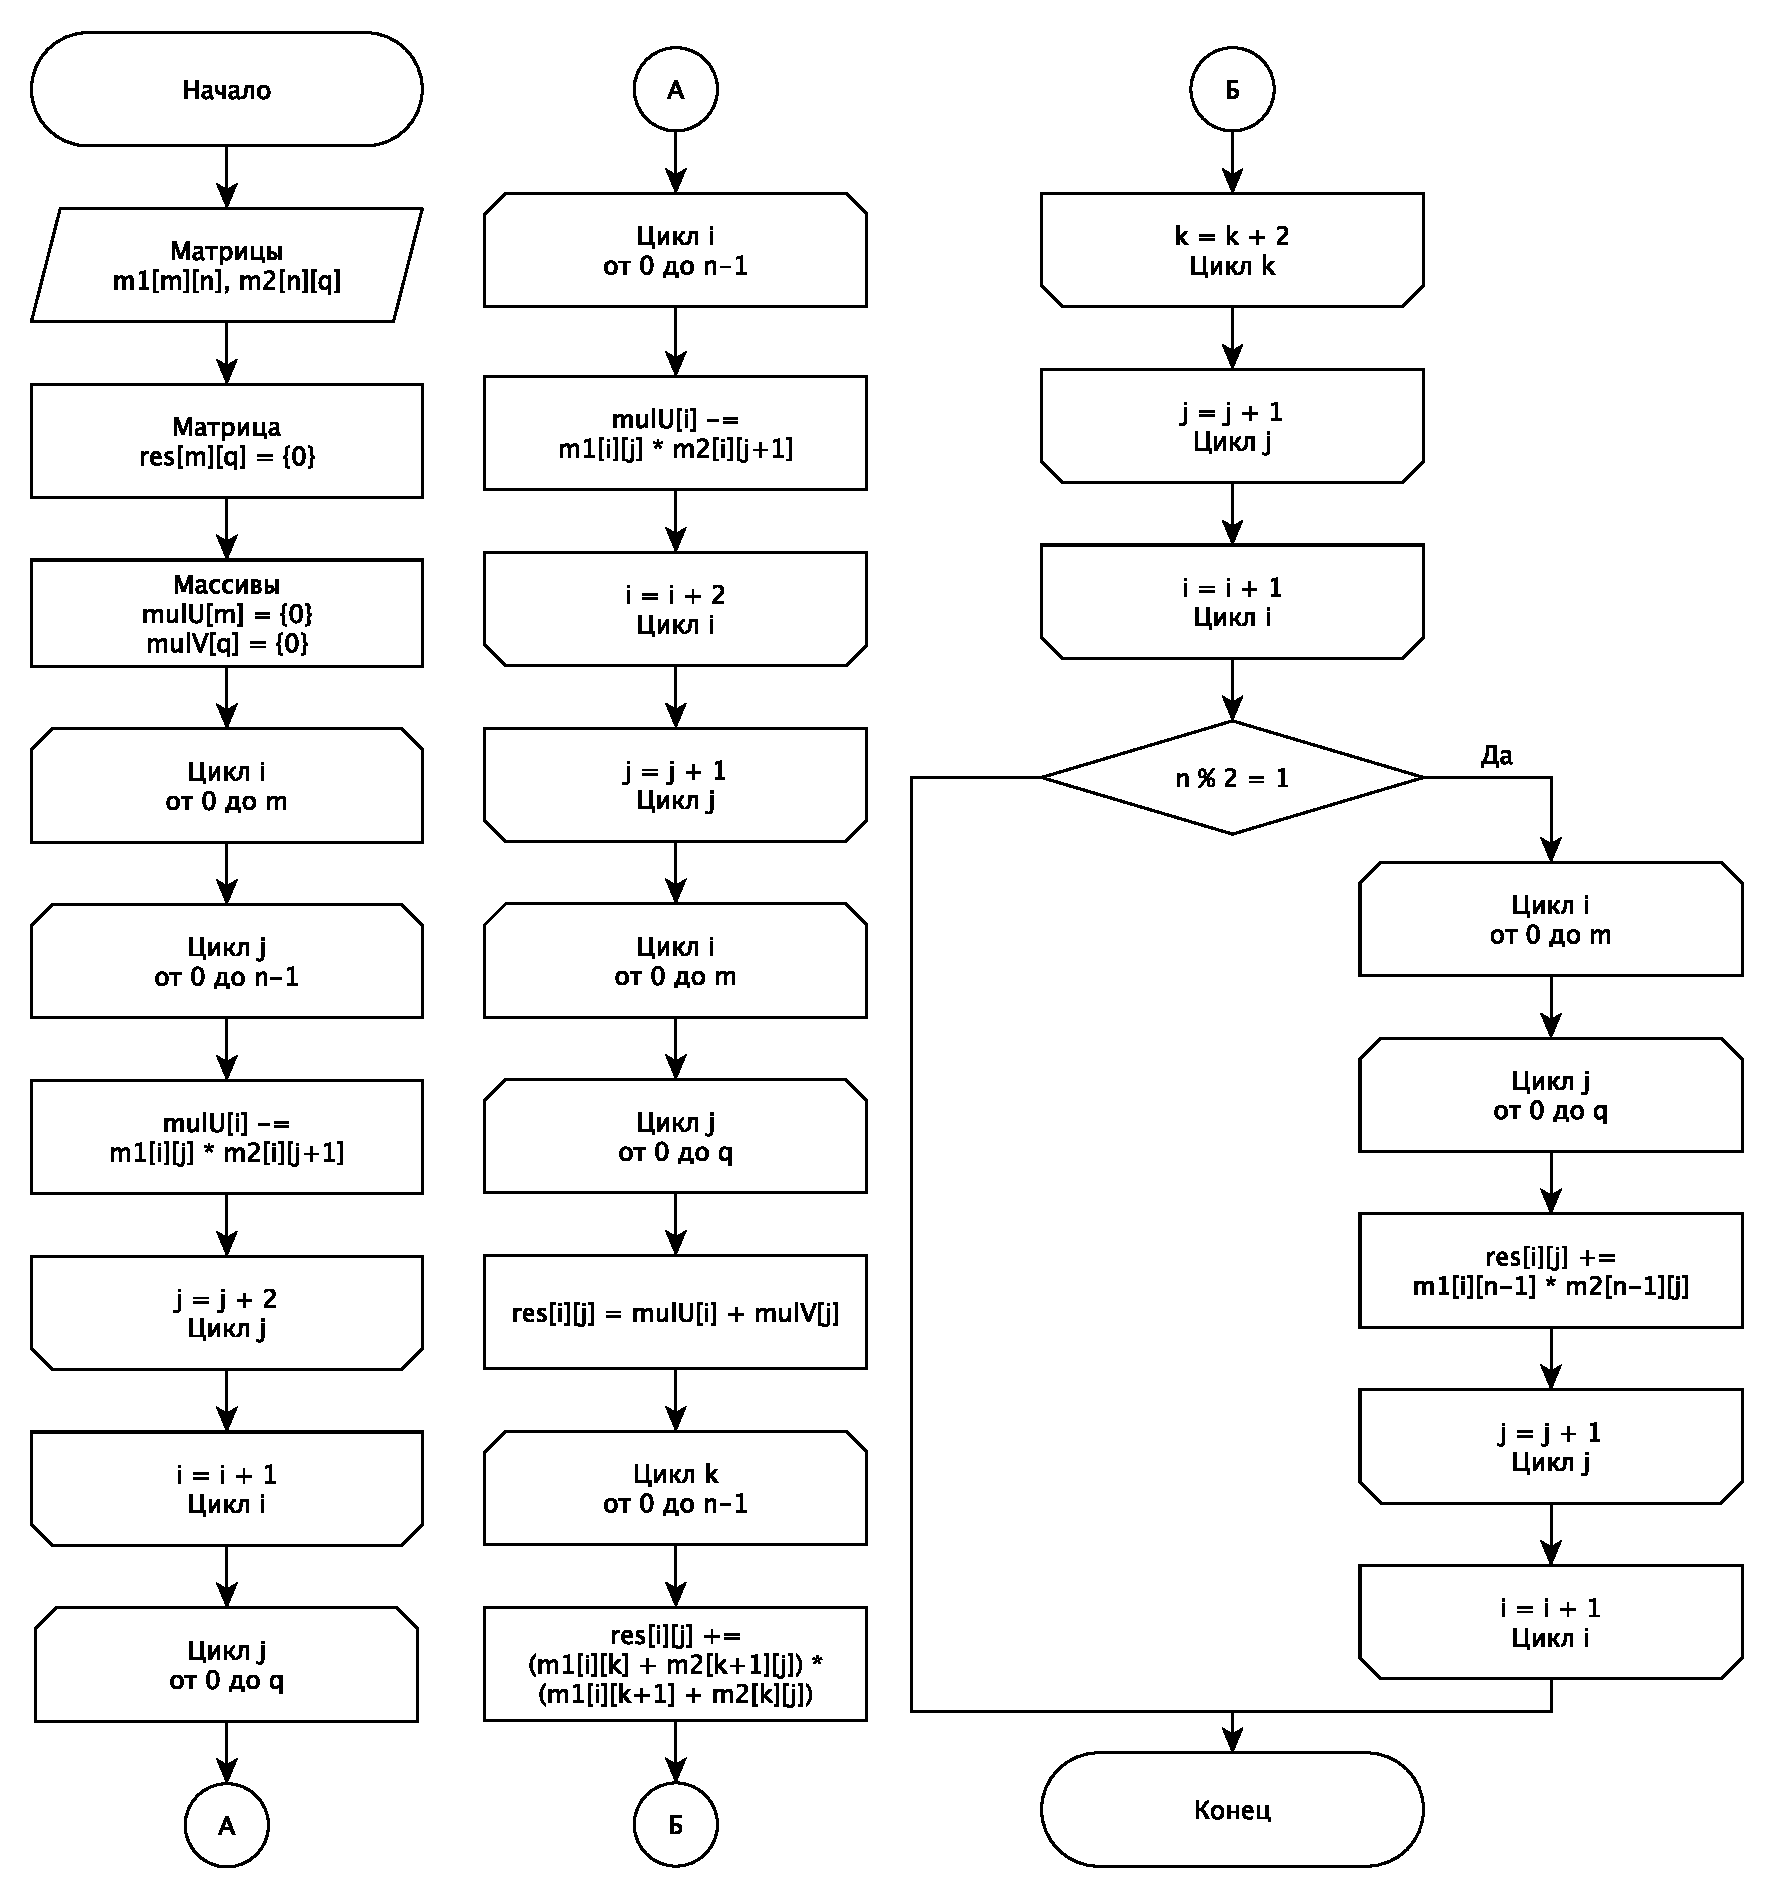
\includegraphics[scale=0.6]{modvinograd}}
    \caption{Схема алгоритма Винограда}
    \label{img:modvinograd}
\end{figure}

На рисунке \ref{img:conveer} представлена схема алгоритма, в котором действия
разделены на конвееры, выполняющиеся в отдельных потоках.

\begin{figure}[H]
    \center{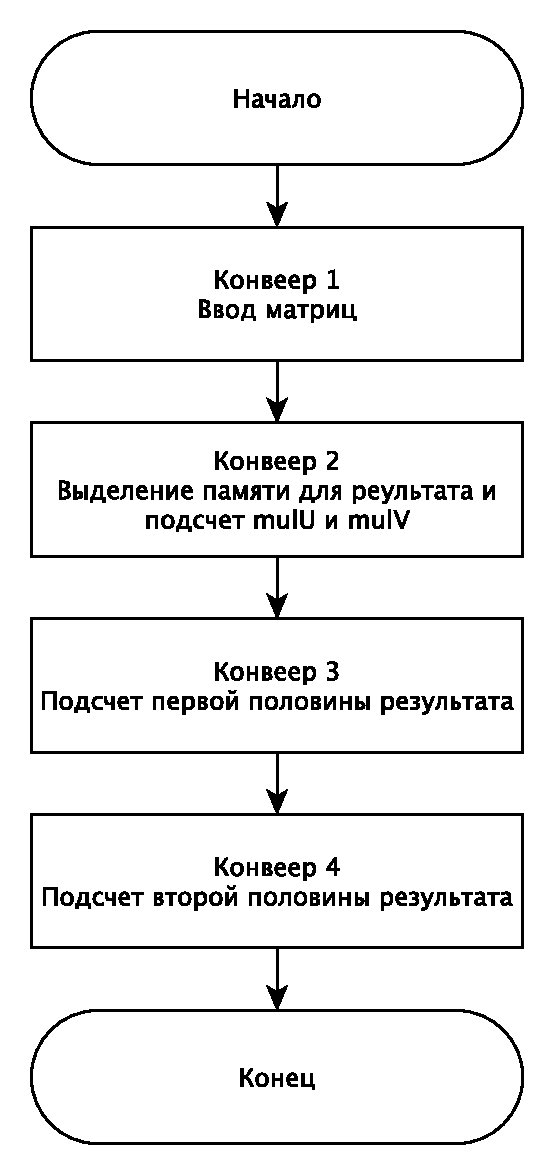
\includegraphics[scale=0.5]{conveer}}
    \caption{Схема конвейера}
    \label{img:conveer}
\end{figure}

\subsection{Выводы}

Описанный принцип построения процессора действительно напоминает конвейер сборочного завода, на котором изделие последовательно проходит ряд рабочих мест. На каждом из этих мест над изделием производится новая операция. Эффект ускорения достигается за счет одновременного выполнения частей алгоритма.
